%!TEX encoding = UTF-8 Unicode 
\documentclass[12pt]{article} 

\usepackage{algorithm}
\usepackage{amsmath}
\usepackage[noend]{algpseudocode}
\makeatletter
\def\BState{\State\hskip-\ALG@thistlm}
\makeatother
\usepackage{graphicx}

%%%%%%%%%%% 頁面與邊界套件 %%%%%%%%%%%
\usepackage[margin = 2cm]{geometry}              %% 邊界為兩公分
\usepackage{fancyhdr}                            %% 無任何頁面設定
    \pagestyle{empty}
\linespread{1.4}                                 %% 1.4 倍原始設定行距
\setlength{\parindent}{0pt}                      %% 不縮排

%%%%%%%%%%%  數學專用套件  %%%%%%%%%%%
\usepackage{amsmath,amssymb,amsfonts}            %% AMS 數學常用符號字型
                                                 %% mathcal, mathfrak, mathbb
\usepackage{mathrsfs,dsfont}                     %% mathscr, mathds
\usepackage{amscd,arcs,esint}                    %% CD 套件/圓弧/積分號
\usepackage[all,cmtip]{xy}                       %% xy-diagram 套件
\usepackage{physics}
\usepackage{color} %red, green, blue, yellow, cyan, magenta, black, white

%%%%%%%%%%%  AMS 定理套件  %%%%%%%%%%%
\usepackage{amsthm}
\usepackage{listings}   
\lstset{breaklines}%这条命令可以让LaTeX自动将长的代码行换行排版
\lstset{extendedchars=false}%这一条命令可以解决代码跨页时,章节标题,页眉等汉字不显示的问题
                      
  \theoremstyle{remark}
  \newtheorem{defi}{Definition}[section]
  \newtheorem{ex}[defi]{範例}
  \newtheorem{thm}[defi]{定理}
  \newtheorem{theorem}{Theorem}
\renewcommand{\proofname}{\sf Pf}
\newenvironment{solution}
  {\renewcommand\qedsymbol{$\blacksquare$}\begin{proof}[Solution]}
  {\end{proof}}

%% 處理 array 行距
%%\renewcommand{\arraystretch}{1.6}

%%%%%%%%%%%  自製特定符號  %%%%%%%%%%%
\def\suchthat{-\hspace{-10pt}\ni\hspace{-10pt}-} %% suchthat
\def\p{\partial}                                 %% partial
\def\pfrac#1#2{\frac{\partial #1}{\partial #2}}  %% 偏微分
\def\contradict{\rightarrow\leftarrow}           %% 矛盾
\def\to{\rightarrow}
\def\abs#1{\left| #1 \right|}                    %% 絕對值
\def\abss#1{\left\| #1 \right\|}                 %% 兩槓
\def\ord#1{\textup{ord}(#1)}
\def\generby#1{\left\langle #1 \right\rangle}    %% generated by ....
\def\geby#1{\generby{#1}}
\def\bN{\mathbb N}
\def\bZ{\mathbb Z}
\def\bQ{\mathbb Q}
\def\bR{\mathbb R}
\def\bC{\mathbb C}
\def\bH{\mathbb H}
\def\bx{\bold x}
\def\by{\bold y}
\def\l{\langle}
\def\r{\rangle}
\def\m{\mu}
\def\a{\alpha}
\def\b{\beta}
\def\bl{\bold l}
\def\bu{\bold u}
\def\bd{\bold d}
  %%CodeColor
\definecolor{mygreen}{RGB}{28,172,0} % color values Red, Green, Blue
\definecolor{mylilas}{RGB}{170,55,241}

\lstset{language=bash,                                                                      %可指定語言種類                                                          
 basicstyle=\ttfamily,                                                       %基本風格
     %keywordstyle=\color{blue},                                                %關鍵字風格
 emph={x,y,z},emphstyle=\color{Orange},                       %其他關鍵字風格(可設定多組)
 emph={[2]a,b,c},emphstyle={[2]\color{blue}},
 commentstyle=\color{red},                                                %註解風格
 stringstyle=\color{Thistle},                                                %字串風格
     %backgroundcolor=\color{SkyBlue},                                %背景風格
 numbers=left,                                                                       %編號
 numberstyle=\tiny,                                                               %編號風格
 numbersep=5pt,                                                                    %編號空格
 %%title=\Huge Particle swarm optimization code,                   %抬頭
}

\usepackage{CJKutf8} 
\begin{document} 
\begin{CJK}{UTF8}{bsmi} 
        %% \begin{center}
    %%\large\sf  2016 Spring, 微積分預覽 lectures notes on ODE
    %% \end{center}
    %% \vspace{-15pt}\hfill {\small Department of mathematics, NTU B00201061 徐唯恩}
    \title{2017 Fall, Numerical Linear Algebra, \\Final project}
    \author{Applied Math \& Electrical Engineering, NTU \\ R05246005 徐唯恩 B03901023 許秉鈞 B03901041 王文謙 R06246001 陳博允}
 
    
 \maketitle{}

 %%%%%%%%%%%%%%%%%%%%%%%%%%1
 \section{Introduction}
What is matrix factorization?
Matrix factorization (MF) factors a sparse rating matrix R ($m$ by $n$, with $N_z$ non-zero elements) into a $m$-by-$f$ and a $f$-by-$n$ matrices, as shown below.
 \begin{figure}[H]
    \begin{center}
        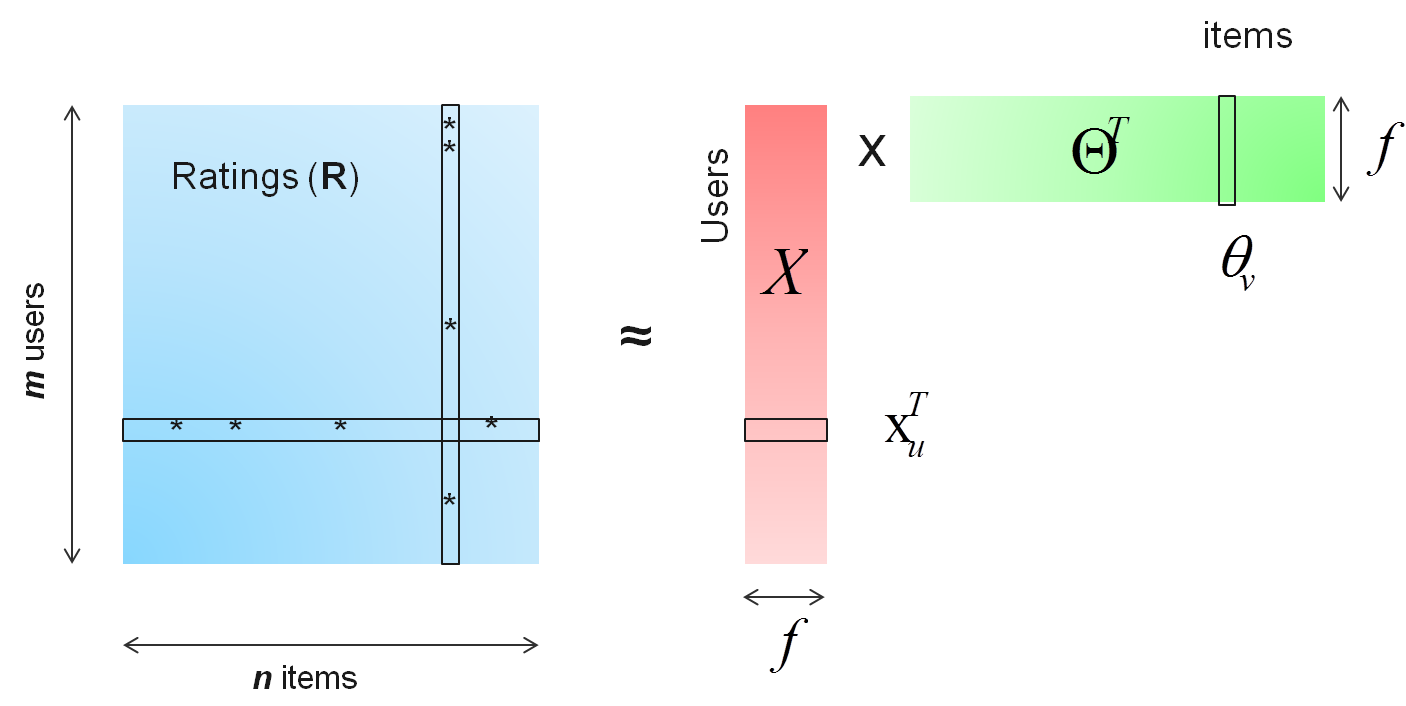
\includegraphics[width=300pt]{1-1.png}
          %\caption{}
        \label{fig:arch_02}
    \end{center}
\end{figure}
Matrix factorization (MF) is at the core of many popular algorithms, e.g., collaborative filtering (https://en.wikipedia.org/wiki/Collaborativefiltering), word embedding, and topic model. GPU (graphics processing units) with massive cores and high intra-chip memory bandwidth sheds light on accelerating MF much further when appropriately exploiting its architectural characteristics.
 \begin{figure}[H]
    \begin{center}
        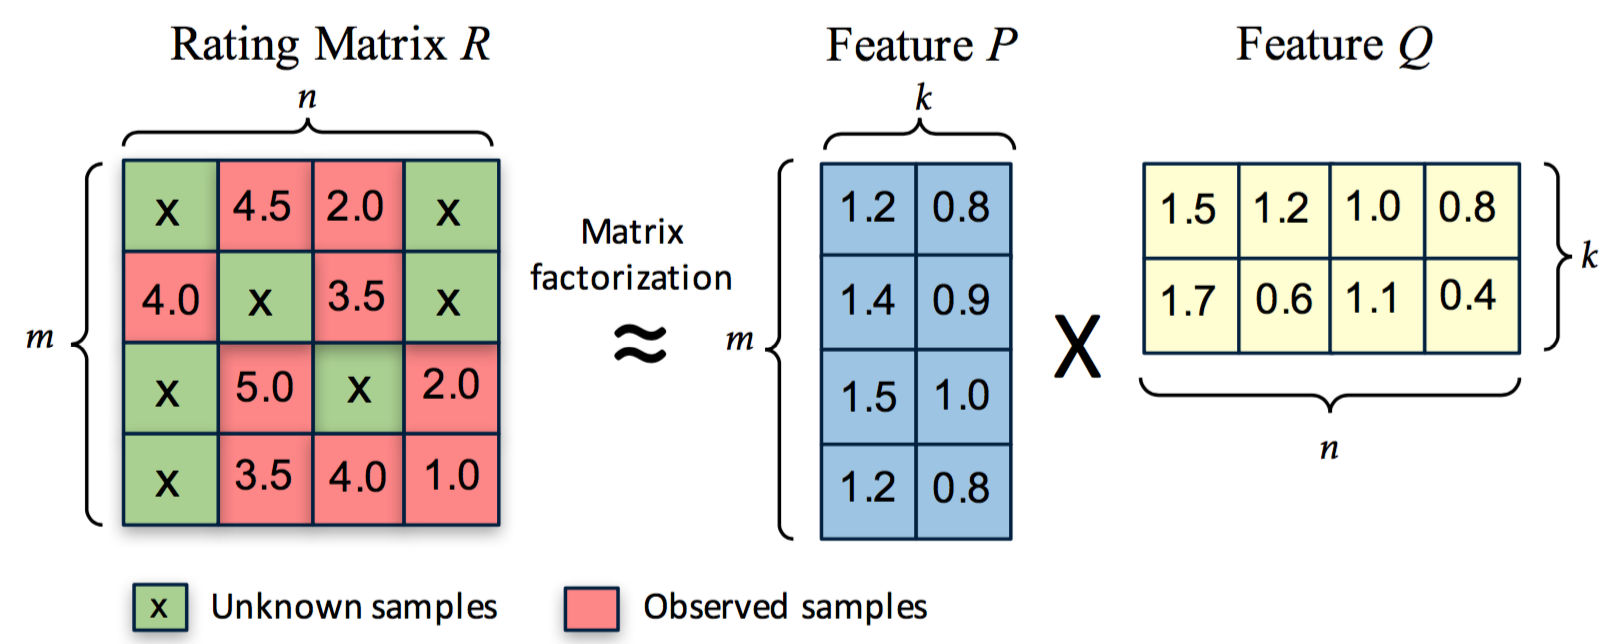
\includegraphics[width=300pt]{1-2.png}
          %\caption{}
        \label{fig:arch_02}
    \end{center}
\end{figure}
Matrix factorization has been demonstrated to be effective in recommender system, topic modeling, word embedding, and other machine learning applications. As the input data set is often large, MF solution are time-consuming. Therefore, how to solve MF problems efficiently is an important problem. \\
Now, we will start from paper reading and the following items are what we have done after paper reading:
\begin{enumerate}
\item Discuss the background of matrix factorization, including that why we do it and what we need to do.
\item Understand the algorithm of non-negative matrix factorization with projected gradient method and the theorems that support to this method.
\item Realize the difference between gradient method and projected gradient method.
\item Read the code (including cuda, cpp, matlab) from the internet and modify these code to fit our data.
\item Write code according to the algorithm in this paper and try to run some bigger data.
\item Compare the results with different parameters. Although there are some data from the internet file of the code are too big to run for our computers, but we still try to make the other data which are smaller and run them successfully.
\end{enumerate}
For the \textbf{item 4 and 5}, we've implemented the \textbf{matlab, C++ CPU version, C++ GPU CUDA verion} of the Projected NMF methods based on some sketchy, fragmented piece of code available on Github, and we will provide links for those references if you're interested. Later on, you can easily see our experimental results and some comparisons with respective to a lot of different parameter settings. You can re-run our experiment based on the \textbf{README} provided in our github repo (\textbf{https://github.com/AdrianHsu/cuMF-final}), which is already attached in the end of this pdf file.\\
Finally we've spent a lot of time dealing with the libraries called \textbf{cuMF-sgd} and \textbf{cuMF-als}, which are the cuda-based libraries that can solve huge problem like Netflix 1GB dataset, or MovieLens 10M dataset. However, the libraries are a bit intricated in that the enviroment set and input data preprocessing, i.e. transform the 3 columns data into COO, CSR format, or binary file in order to speed up.
%%%%%%%%%%%%%%%%%%%%%%%%%%2
 \section{Paper reading and comprehension}
We first start from reading the paper Projected Methods for Non-negative Matrix Factorization (CJ Lin, 2005). The reason why we choose this paper is that the factorization a nonnegative matrix is needed in recommendation system. Thus we will state and show the algorithm as detail as possible. Now, we have a core problem is that given a nonnegative matrix $V_{n\times m}$ to find two nonnegative matrices $W_{n \times r},H_{r \times m}$ such that 
$$V=WH.$$ 
However, we cannot ensure that the equility always holds. So, the problem can be convert to an optimal problem in several ways. One way is as follow. 
\subsection{Some existing methods for matrix factorization}
Given $f : \bR^{n\times r} \times \bR^{r\times m } \to \bR$ which is defined as 
$$
f(W,H) := \frac{1}{2}\sum_{i=1}^n \sum_{j=1}^m ( V_{ij} - (WH)_{ij} )^2,
$$
where the factor $\frac{1}{2}$ is for convenience to operate the gradient differentiation. In fact, it is exact half of square of Frobenius norm of $V-WH$, that is 
$$
\sum_{i=1}^n \sum_{j=1}^m ( V_{ij} - (WH)_{ij} )^2 = \norm{V-WH}^2_F
$$
So what we want to find is the to optimal
$$
\min_{W,H} f(W,H) = \min_{W,H}  \sum_{i=1}^n \sum_{j=1}^m ( V_{ij} - (WH)_{ij} )^2 
$$ which is subject to $W_{ia}\geq 0 , H_{bj}\geq 0$, $\forall i,a,b,j$. \\
Sure, there are some other methods to convert such as an "entropy like" method, that is
$$
\min_{W,H} \left( \sum_{i=1}^n\sum_{j=1}^m \left( V_{ij}\log{\frac{V_{ij}}{WH_{ij}} - V_{ij} +(WH)_{ij} } \right) \right).
$$
Also, there are some nontrivial properties but not used in this paper, so we skip these detail in existing methods.
\subsection{Explain how projective gradient method works }
Now we will see the projective gradient methods for bound-constrained optimization. Consider the following standard form of bound-constrained optimization problem.\\ 
Let $f:\bR^{n}\to \bR$ is a continuous differentiable function, and $\bl ,\bu$ are lower and upper bound-constrains. Assume $k$ is the index of iterations.
$$
\min _{x\in \bR^n} f(x)
$$
subject to $l_i \leq x_i \leq u_i$ for $i=1,2,...,n$. 
Now we are going to explain why the minimum will occurs. And in section (2.3), we will explain the how Projective Gradient Method apply to nonnegative matrix factorization and how its algorithm comes.

\subsection{Proof of existence of the projective gradient method}
In this paper, there is no proof of existence of the projective gradient method. First of all, we assume that we are process an optimization problem in a convex domain. In particular, $\bR^n$ is convex set. Now we consider the problem
$$
\min_{x\in S} f(x),
$$
where $S$ is a nonempty closed convex set. We want to prove there exist a projection operator $P_S(x)$ which can calculate the minimum $\arg \min_{y \in S}\norm{x-y}$ . In fact, Projected Gradient Method is a simple method which modify the Gradient Method by the projection process. One can prove that the convergence and convergent rate is closed to Gradient Descent. Now we want to show the existence and uniqueness of projection matrix. 
\begin{theorem}
If $S\subset \bR^n$ is a nonempty closed convex set, then for any $x\in \bR^n$,
$$
\min_{y\in S} \norm{x-y}
$$
exists a unique solution $x_S$. And $x_S$ is the optimal solution if and only if $(x-x_S)^T(y-x_s)\leq 0$, $\forall y \in S$.
\end{theorem}
\begin{proof}
Let $x'\in S$, and consider a ball $B_{\norm{x-x'}}(x)$. Then $S\cap B_{\norm{x-x'}}(x)$ is nonempty and convex, thus it follows the existence.\\
For second part, if $x\in S$, naturally the optimal solution $x_S=x$. Conversely, $(x-x_S)^T(y-x_s)\leq 0$ and $x\in S$ imply $\norm{x-x_S}^2\neq 0$ and hence the necessary and sufficiency holds. The other case if $x\notin S$, we prove the necessary first by contradiction. Suppose $x_S$ is a projection point and the inequality doesn't hold. So there exist $y \in S$ such that $(x-x_S)^T(y-x_s) > 0$. Now consider $x_\theta = x_S + \theta(y-x_S)$, where $\theta \in [0,1]$. And by the convexity, we get $x_\theta \in S$. Consider
$$
\norm{ x-x_\theta }^2 = \norm{ x-x_S -\theta(y-x_S)  }^2 = \norm{ x-x_S  }^2 -2\theta (x-x_S)^T(y-x_S) + \theta^2 \norm{y-x_S}^2
$$
Since $\theta^2$ approaches to zero faster than $\theta$ as $\theta \to 0$. So
$$
-2\theta (x-x_S)^T(y-x_S) + \theta^2 \norm{y-x_S}^2 < 0
$$ 
whenever $\theta$ small enough. Hence get a contraction. Second, we prove the sufficiency. Suppose the inequality always holds $\forall y \in S$. To prove $x_S$ is the optimal solution, consider for any $y\in S$, we have
\begin{eqnarray*}
\norm{x-y}^2 &=& \norm{ x-x_S +x_S -y }^2\\
 &=& \norm{x-x_S}^2 -2 (x-x_S)^T(y-x_S)+ \norm{x_S-y}^2\\
 &\geq& \norm{ x-x_S  }^2 + \norm{x_S-y}^2
\end{eqnarray*}
So we get that as $y\neq x_S$, $\norm{x_S-y}^2>0$, and so $\norm{x-y}^2 > \norm{x-x_S}^2$. And since $y$ is arbitrary. So we proved that $x_S$ is optimal solution.
\end{proof}
Now we consider the nonnegative cone: $ S := \left\{ x | x\geq0 \right\}$ we only project from each dimension to nonnegative semi axis, that is $x_i \leftarrow \max{\left\{ x_i,0 \right\}}$. Now we go back to the Projected Gradient Method. Assume we have a blackbox can easily compute $P_S(x)$, then we only need to process follows to convergent.
\begin{eqnarray*}
\bar{x_k} &=& P_S(x_k-s_k\grad f(x_k)),s_k>0\\
x_{k+1}   &=& x_k + \alpha_k(\bar{x_k}-x_k),\alpha_k \in ( 0,1],
\end{eqnarray*}
where $s_k>0$ is a step size parameter. And thus the iterated algorithm as follow
$$
x_{k+1} = P_S(x_k-s_k \grad f(x_k)   ). 
$$
That is a combination of common gradient descent and projection operator $P_S(\dot)$ in some feasible set. And the parameter $\alpha$ is a step size of choice of line search. We demand $\alpha_k \in ( 0,1]$ can make sure next $x$ will not go out of feasible set. By the property of Gradient Descent which has a fixed step size:
$$
\norm{ x_{k+1}-x*} \leq M \norm{x_k -x* },
$$ 
where $x*$ is the optimal solution and $M \in (0,1) $.  
So in the Projected Gradient Method. We have the same inequality as above. And we get
\begin{eqnarray*}
\norm{P_S(x_{k+1}-x*)} &=& \norm{ P_S(x_{k+1})-P_S(x*) } \\
 &\leq& \norm{ x_{k+1} - x* }\\
 &\leq& M \norm{x_k-x*}
\end{eqnarray*}
Finally, we prove the contraction of the projection operator.
\begin{theorem}
Let $S\subset \bR^n$ is a nonempty closed convex set, then the projection operator
$$
P_S:x \mapsto \arg \min_{y \in S}  \norm{x-y}, \forall x,y\in \bR^n
$$
\end{theorem}
\begin{proof}
Consider $x,y$ and their projection $x_S,y_S$. Let $H_x,H_y$ are hyperplanes passing through $x_S,y_S$ and with the normal vector $x_S-y_S$. So we know the distance of two hyperplanes is $\norm{x_S-y_S}$. By Theorem1, we know $x,y$ are either in the hyperplane or out of the hyperplane. Thus the theorem2 follows.
\end{proof}
By the previous conclusion, the projection operator is a contraction, so though we add a projection precess, it will not change the convergence of original Gradient Method.

\subsection{Projected Gradient Method for NMF}
We use the same optimization problem as (2.1) mentioned, that is
$$
f(W,H) := \frac{1}{2}\sum_{i=1}^n \sum_{j=1}^m ( V_{ij} - (WH)_{ij} )^2,
$$
Now, we calculate the gradient
$$
\grad_Hf(W,H)=W^T(WH-V).
$$
At each iteration, we can find a step size $\alpha$ by algorithm (4) in this paper. This algorithm satis equation
\begin{equation}
f(x^{k+1})-f(x^k) \leq \sigma \grad f(x^k)^T (x^{k+1}-x^k).
\end{equation}
And check whether the current solution
$$
\tilde{H}:= P[H-\alpha \grad f(H)]
$$
satisfies above equation or not.
The other hand, consider the quadratic function $f(x)$ and any vector $\bold d$, we have
$$
f(x+ \bd) = f(x) + \grad f(x)^T \bd + \frac{1}{2}\bd^T\grad^2f(x)\bd.
$$
Then for two consecutive iterations $\bar{x}$ and $\tilde{x}$, equation (1) can be rewritten as
$$
(1-\sigma)\grad f(\bar{x})^T ( \tilde{x} - \bar{x} )+ \frac{1}{2}( \tilde{x} - \bar{x} )^T\grad^2f(\bar{x})( \tilde{x} - \bar{x} ) \leq 0.
$$
As put $H$ into $x$, we have
$$
(1-\sigma) \l \grad f(\bar{H}), \tilde{H}-\bar{H} \r+\frac{1}{2} \l \tilde{H}-\bar{H},W^TW(\tilde{H}-\bar{H}) \r \leq 0
$$
Also, we can use the same procedure to update $W$.

\subsection{Stopping Condition}
Finally, the last main idea is in the section 5 this paper, the left section 6 and 7 are some numerical experiments. In this section, we make the algorithm stop when the numbers of iteration achieve to the given limit or the difference between recent iterations small enough. For the second item, a common condition to check if a point $x^k$ is close to a stationary point for bound-constraint optimization is
\begin{equation}
\norm{ \grad^pf(x^k)} \leq \epsilon \norm{ \grad f(x^1) } ,
\end{equation}
where $\grad^pf(x^k)$ is the projected gradient defined as
\[
\grad ^pf(x^k)_i := \left\{\begin{array}{ll}

                 \grad f(x)_i & \mbox{if $l_i<x_i<u_i)$} \\  % 文字的部份要用 \mbox
                 \min \left\{ 0,\grad f(x)_i \right\}, & \mbox{if $x_i=l_i$} \\  % 包住,讓他使用正常字體
                 \max \left\{ 0 , \grad f(x)_i\right\},      & \mbox{if $x_i=u_i$}
                \end{array} \right.
\]
which follows from an equivalent form of the KKT condition for bounded problem and
$$
\norm{ \grad^pf(x)}=0
$$
The other hand, for NMF, equation (2) becomes
$$
\norm{ \grad^pf(W^k,H^k)}_F \leq \epsilon \norm{ \grad f(W^1,H^!) }_F.
$$
Notice that the tolerance of the sub-problem should not be the same as the global one but relatively, i.e. The return matrices $W^{k+1}$ and $H^{k+1}$ from the sub-problem should respective satisfy
\begin{eqnarray*}
\norm{ \grad^p f(W^{k+1},H^{k}) }_F &\leq& \bar{ \epsilon}_W\\
\norm{ \grad^p f(W^{k+1},H^{k+1}) }_F &\leq& \bar{ \epsilon}_H,
\end{eqnarray*} 
where we set 
$$
\bar{ \epsilon}_H = \bar{ \epsilon}_W=\max \left\{10^{-3},\epsilon \right\} \cdot \norm{ \grad f(W^1,H^1) }_F
$$
with given $\epsilon$ in the beginning. If, unfortunately, the projected gradient method complete without any iterations, we decrease the stopping tolerance by
$$
\bar{\epsilon}_W \leftarrow \frac{\bar{\epsilon}_W}{10}
$$
and $\bar{\epsilon}_H$ is reduced in a similar way for the sub-problem.
%%%%%%%%%%%%%%%%%%%%%%%%%%3
 \section{Experiments}
\subsection{ how dimension R affects the convergence}
This experiment describes about how the dimension R in M*R*N affects the convergence. We use the MovieLens 100K datasets which is (943, 1682), and the nnz = 100000. 
As the table shows, we can discover that as R goes larger, the will affect the projection norm in the final round, and if the tolerance is larger, the norm will be larger in the final round. However, even if the norm changes drastically, we can still discover that the Frobenious norm still remains, around 1000.00
\begin{figure}[H]
    \begin{center}
        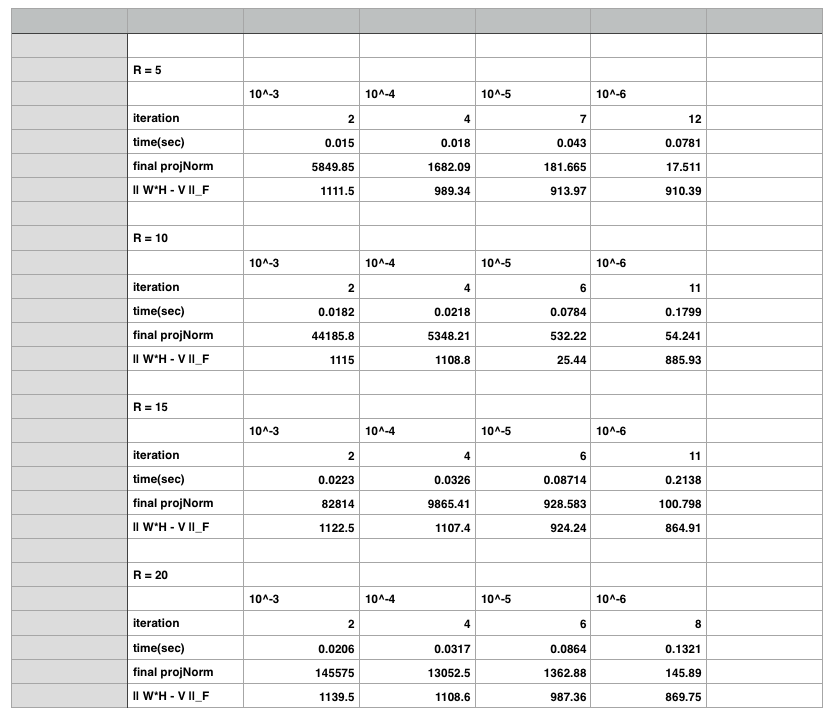
\includegraphics[width=500pt]{dimensionR.png}
          %\caption{}
        \label{fig:arch_02}
    \end{center}
\end{figure}

\subsection{ how dimension M,N affects the convergence}
For this experiment, we want to discuss about the correlation between the dimension M, N will affect the number of iterations, and the total time... etc. As the table shows, we find that when M and N is around 100, and then we fix the tolerance, we can see that the Final projForm and Frobenius norm, the value are heavily depend on the M nad M; however, the number of iterations remain almost the same even though the matrix is very large.
\begin{figure}[H]
    \begin{center}
        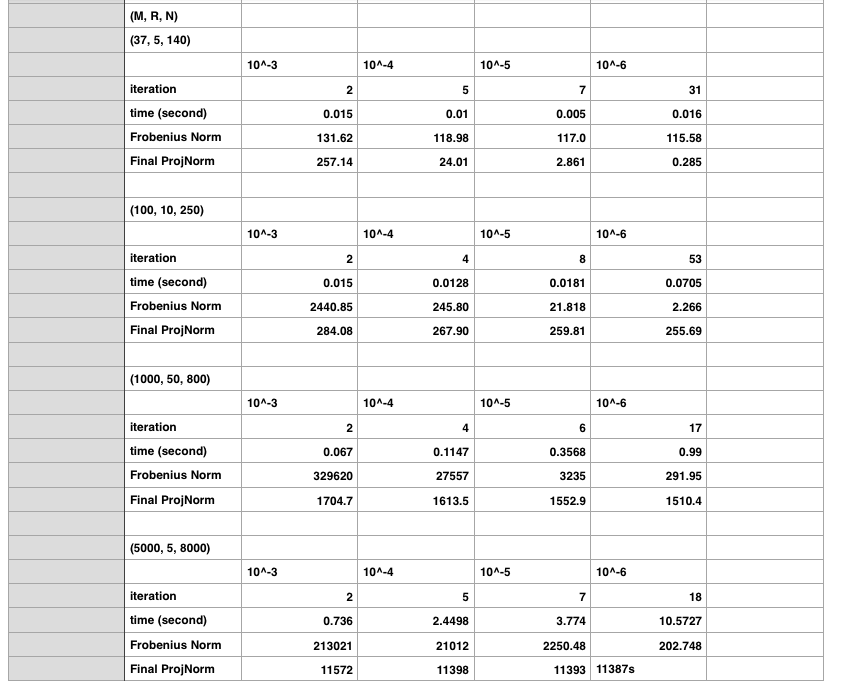
\includegraphics[width=500pt]{dimensionMN.png}
          %\caption{}
        \label{fig:arch_02}
    \end{center}
\end{figure}

\subsection{GPU v.s. CPU w.r.t memory and time}
For this subsection, we will consider the dataset named \textbf{Movie Lens 100K} that contains 100000 nnz and the $M = 943$, $N = 2625$, which is not so large but still have some interesting properties that we can investigate. If you want to re-implement this experiment, you can download the code on Github and then fetch the data from here: \textbf{konect.uni-koblenz.de/networks/movielens-100k\_rating}. This dataset is also provided in the README file, so you can get the link in my repo.

\mbox{} 
\begin{lstlisting}
~/nla/pgrad-2$ ./NMF ml100k.txt
GPU Device 0: Tesla K80 with compute capability 3.7
Init gradient norm 7348422.314490
tol*initgrad = 7.348422
Iter = 1 Final proj-grad norm 8008612.469400
Iter = 2 Final proj-grad norm 112.232496
Iter = 3 Final proj-grad norm 472.571561
Iter = 4 Final proj-grad norm 1.020186
values in W*H (column major) are:
The ||W*H-V||_F is: 1066.802909
total elapsed time:
user	0m24.912s
sys	0m8.120s
=== CPU version (tol = 1e-7) ===
/tmp3/4dr14nh5u/nla/cpu$ ./setup.sh ml100k.txt
Init gradient norm 64382280.742422
tol*initgrad = 6.438228
Iter = 1 Final proj-grad norm 64382280.742422
Iter = 2 Final proj-grad norm 0.650105
Iter = 3 Final proj-grad norm 0.650105
The result W*H is
The ||W*H-V|| is: 1076.549118
total elapsed time:
user	0m1.620s
sys	0m0.020s
=== CPU version (tol = 1e-9) ===
/tmp3/4dr14nh5u/nla/cpu$ ./setup.sh ml100k.txt
Init gradient norm 64382280.742422
tol*initgrad = 0.064382
Iter = 1 Final proj-grad norm 64382280.742422
Iter = 2 Final proj-grad norm 0.650105
Iter = 3 Final proj-grad norm 1.516980
Iter = 4 Final proj-grad norm 3.809543
Iter = 5 Final proj-grad norm 685.653741
Iter = 6 Final proj-grad norm 182.464007
... (we shut down this since that it is overfitting)
The ||W*H-V||_F is: 984.109280
total elapsed time:
user	0m13.291s per round (but not always stay like this)
sys	0m0.039s
\end{lstlisting}
\mbox{} \\

We can easily discover that the CPU version is performing better than the GPU version, which is abnormal. As what we've discovered, the reason is that for CUDA, we have to use cudaMalloc(), cudaFree() and a lot of memory operation for GPU version, however in CPU version you can perform the linear algebra operation directly on stack Memory. Nevertheless, we have confidence that if we can try on larger dataset, (given that we solved the memory not-enough problem, please see the chapter talked about what problem we have encountered)for example, Netflix 1G dataset, and utilizing the BLOCK and THREAD in cuda programming, we can found that the GPU verion perform better if data grows larger.

%%%%%%%%%%%%%%%%%%%%%%%%%%4
\section{Comparison of cuMF Libraries}
\begin{figure}[H]
    \begin{center}
        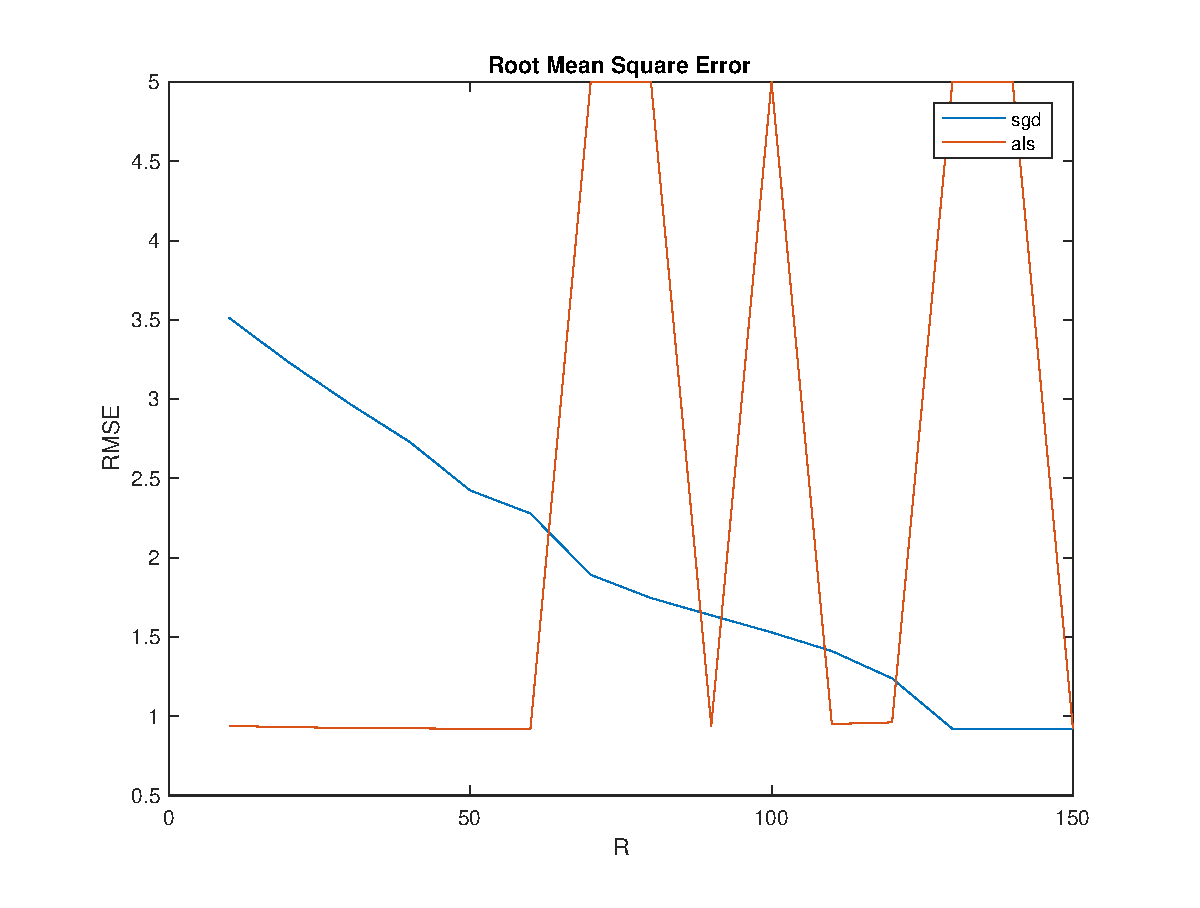
\includegraphics[width=500pt]{rmse.eps}
          %\caption{}
        \label{fig:arch_02}
    \end{center}
\end{figure}
In the first plot, we compare the execution time with different R between cumf\_als and cumf\_sgd methods.  It is reasonable that the execution time increase as R become greater because of the data to be processed increase, but surprisingly the execution time seems to have nothing to do with R increase in the SGD method. On the other hand, the execution time by the cumf\_sgd method is overall less than that of the cumf\_als method.
\begin{figure}[H]
    \begin{center}
        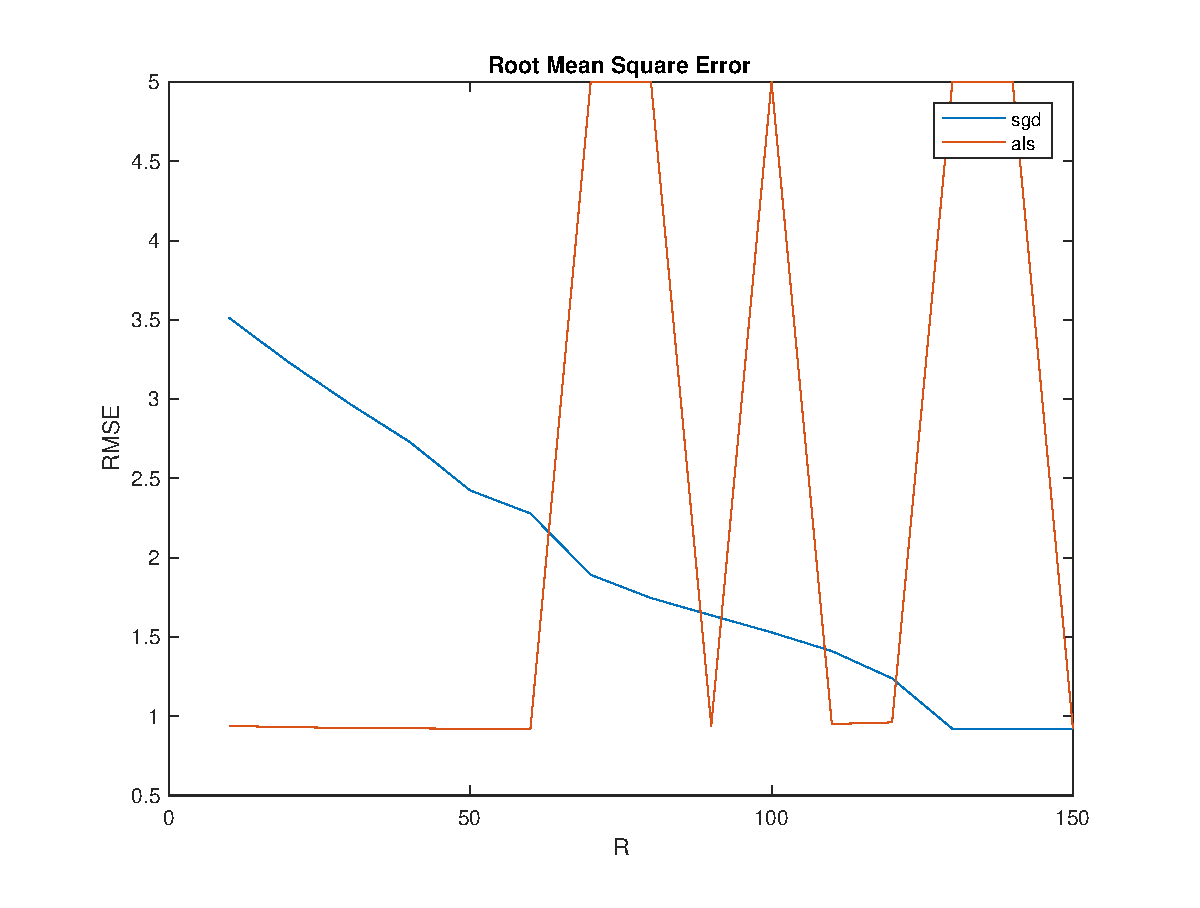
\includegraphics[width=500pt]{time.eps}
          %\caption{}
        \label{fig:arch_02}
    \end{center}
\end{figure}
In the second plot, we compare the RMSE(Root Mean Square Error) between the two methods.  There are some aspects that can be observed in this plot.  First of all, the RMSE in cumf\_als method will diverge in some $R$ (The RMSE result in the program outputs NaN, and we set these result as 5 for the sake of better\-look in this plot) although the diversity hasn’t been mentioned in the paper.

  The reason of this property, we guess, is that when we calculate the $Ax=b$, the singularity of $A$ could approach 0(ill-conditioned).  This may result in the components in $A^{-1}$ becomes large when we take inverse of $A$.  Second, the RMSEs for cumf\_sgd method are larger than that of cumf\_als in small $R$, but it gradually decreases while $R$ increase and approach the RMSEs of cumf\_als, if it doesn’t diverge, of course.
%%%%%%%%%%%%%%%%%%%%%%%%%%5
 \section{Difficulties and Challenges}
During our implementation process and the environment setting such as installing CBLAS, CUBLAS, CMAKE...etc, We've encountered a lot of difficulties. Ine problem is that the data type "double" in C/C++ cannot handle such large number, and therefore we slightly modified the data so that it is more adaptable toward our model.\\
The other problem we've encountered is that we don't have to transform our initial matrix from dense to the sparse one, because we have to admit that we've spent too much time dealing with the environment setting and getting familiar with the c memory allocation, and cuda memory allocation. Therefore if the matrix is too large, such as M = 1E6, and also N = 1E6, and then our matrix cannot contain these data, since that our 2-D array is too small to being performing and multiplication or dot product on them.
%%%%%%%%%%%%%%%%%%%%%%%%%%6
\section{References}
\textbf{1. Xiaolong Xie, Wei Tan, Liana Fong, Yun Liang, CuMFSGD: Parallelized Stochastic Gradient Descent for Matrix Factorization on GPUs.}
\\
\textbf{2. Faster and Cheaper: Parallelizing Large-Scale Matrix Factorization on GPUs. Wei Tan, Liangliang Cao, Liana Fong}.
\\
\textbf{3. NMF.cu}: This code solves NMF by alternative non-negative least squares using projected gradients. It's an implementation of \textbf{Projected gradient methods for non-negative matrix factorization} by CJ Lin. You may read the paper for more details.
\\

\end{CJK} 
\end{document}